--Explain the tool from a high-level point of view--

This work presents  \toolName\ (Multi-robot plAnner for PArtially Known EnviRonments), a \emph{novel} \emph{decentralized} planner for partially known environments.
%\toolName\ modifies~\cite{tumova2016multi} by supporting partial knowledge.
Given a team of robots and a local mission for each robot, \toolName\ partitions the set of robots into classes based on dependencies dictated by the local missions of each robot.
For each of these classes, it explores the state space of the environment and the models of the robot searching for definitive and possible plans.
A \emph{definitive plan} is a sequence of actions that ensure the satisfaction of the local mission for each robot.
A \emph{possible plan} is a sequence of actions that may satisfy the local mission due to some unknown information about the model of the robots or the environment in which they are deployed.
\toolName\ chooses the plan that allows the achievement of the mission by performing the lower number of actions, but other policies can also be used.


\textbf{Specific contributions.} Specific contributions are detailed in the following:
\begin{enumerate*}
\item we define the concept of \emph{partial robot model}, which allows the description of the behavior of the robots and its environment when only partial information is available. 
Specifically, a partial robot model allows considering three types of partial information: partial knowledge about the execution of transitions (possibility of changing the robot location), on service provision (whether the execution of an action succeed in providing a service) and on the meeting capabilities (whether a robot can meet with another);
%\item we define two possible LTL semantics on paths namely three-valued and thorough path semantics  and prove that  two semantics are particular cases of the more general thorough semantics~\cite{bruns2000model};
\item we define the concept of local mission satisfaction for partial robot models;
\item we define the distributed planning problem for partially specified robots;
\item we propose a distributed planning algorithm and we proved its correctness;
%\item we evaluate the proposed algorithm on a robot application obtained from the RobotCup Logistics League competition~\cite{karrasrobocup} andon a robotic application working in an apartment of about 80 m$^2$, which is part of a large residential facility for senior citizens~\cite{map}.
The results show the effectiveness of the proposed algorithm.
\end{enumerate*}

The presence of partial knowledge about the robots and their environment is described in the following.

\textbf{Partial knowledge about the actions execution.} 
The robots can move between cells separated by grey lines, while they cannot cross black bold lines.
It is unknown whether it is possible to move between cells $c_{14}$ and $c_{20}$.
This is indicated using a dashed black bold line.
It is also unknown whether robot $r_3$ can send pictures using a communication network in location $l_3$ and specifically in cell $c_{18}$, i.e., whether action $s_p$ can be performed. 
Locations of the environment where it is unknown if an action can be provided are marked with the name of the action preceded by symbol $?$.

\textbf{Unknown service provisioning.} 
There are cases in which actions can be executed but there is uncertainty about service provisions.
For example, actions $ud1$ and $ud2$ of robot $r_2$ unload the robot.
Action $ud2$ will always be able to provide the \emph{unload} service, while it is unknown whether $ud1$ is actually able to provide this service since its effectiveness depends on the size of the collected debris. 
In Fig.~\ref{fig:example1}, the label $L(ud1,unload)=?$ indicates that there is partial knowledge about the provision of the \emph{unload} service when action $ud1$ is performed. 

\textbf{Unknown meeting capabilities.} 
It is  unknown whether robots $r_1$ and $r_2$ can meet in one cell of the environment. 
For example,  $r1$ to load $r2$ cannot concurrently execute services $ld$ and $rd$. 
Unknown meeting capabilities are indicated with rotating arrows labeled with the symbol $?$.
For example,  in Fig.~\ref{fig:example1}, it is unknown whether robots $r_1$ and $r_2$ are able to meet in cell $c_{9}$.

An overview of \toolName\ is depicted in ~\ref{fig:overview}.
The \emph{Planner} script uses the models of the robot(s) and the environment in order to compute the path-planning.
The model of each robot contains information regarding its initial position, the number of services and their location that the robot must perform and the locations where the modeled robot has to synchronize with another one.  
The model of the environment depicts its map and defines the allowance of transitions between the cells that compound the model.
This two models must be manually defined but can be reused for an infinite number of experiments.
Then, the \emph{Random model generator} generates a certain number (defined by the user) of tests based on the previously explained models.
Each of this tests is unique since the generator associates a random uncertainty and initial position of the robotic team to each of them.
This process is performed for each experiment, since the uncertainty that is checked changes between them (e.g. execution of transitions in Experiment 1, services provisioning in Experiment 2 and meeting capabilities in Experiment 3).
The generation of models must be performed once, although we provide an already working set in our repository and this step can be skipped.
This set is stored in the folder "ReplicationPackage", where the new scenarios must be saved as well.

Once the models are set, the planner can be executed selecting the suitable number of experiment and research question to be checked.

\begin{figure}[!t]
\begin{center}
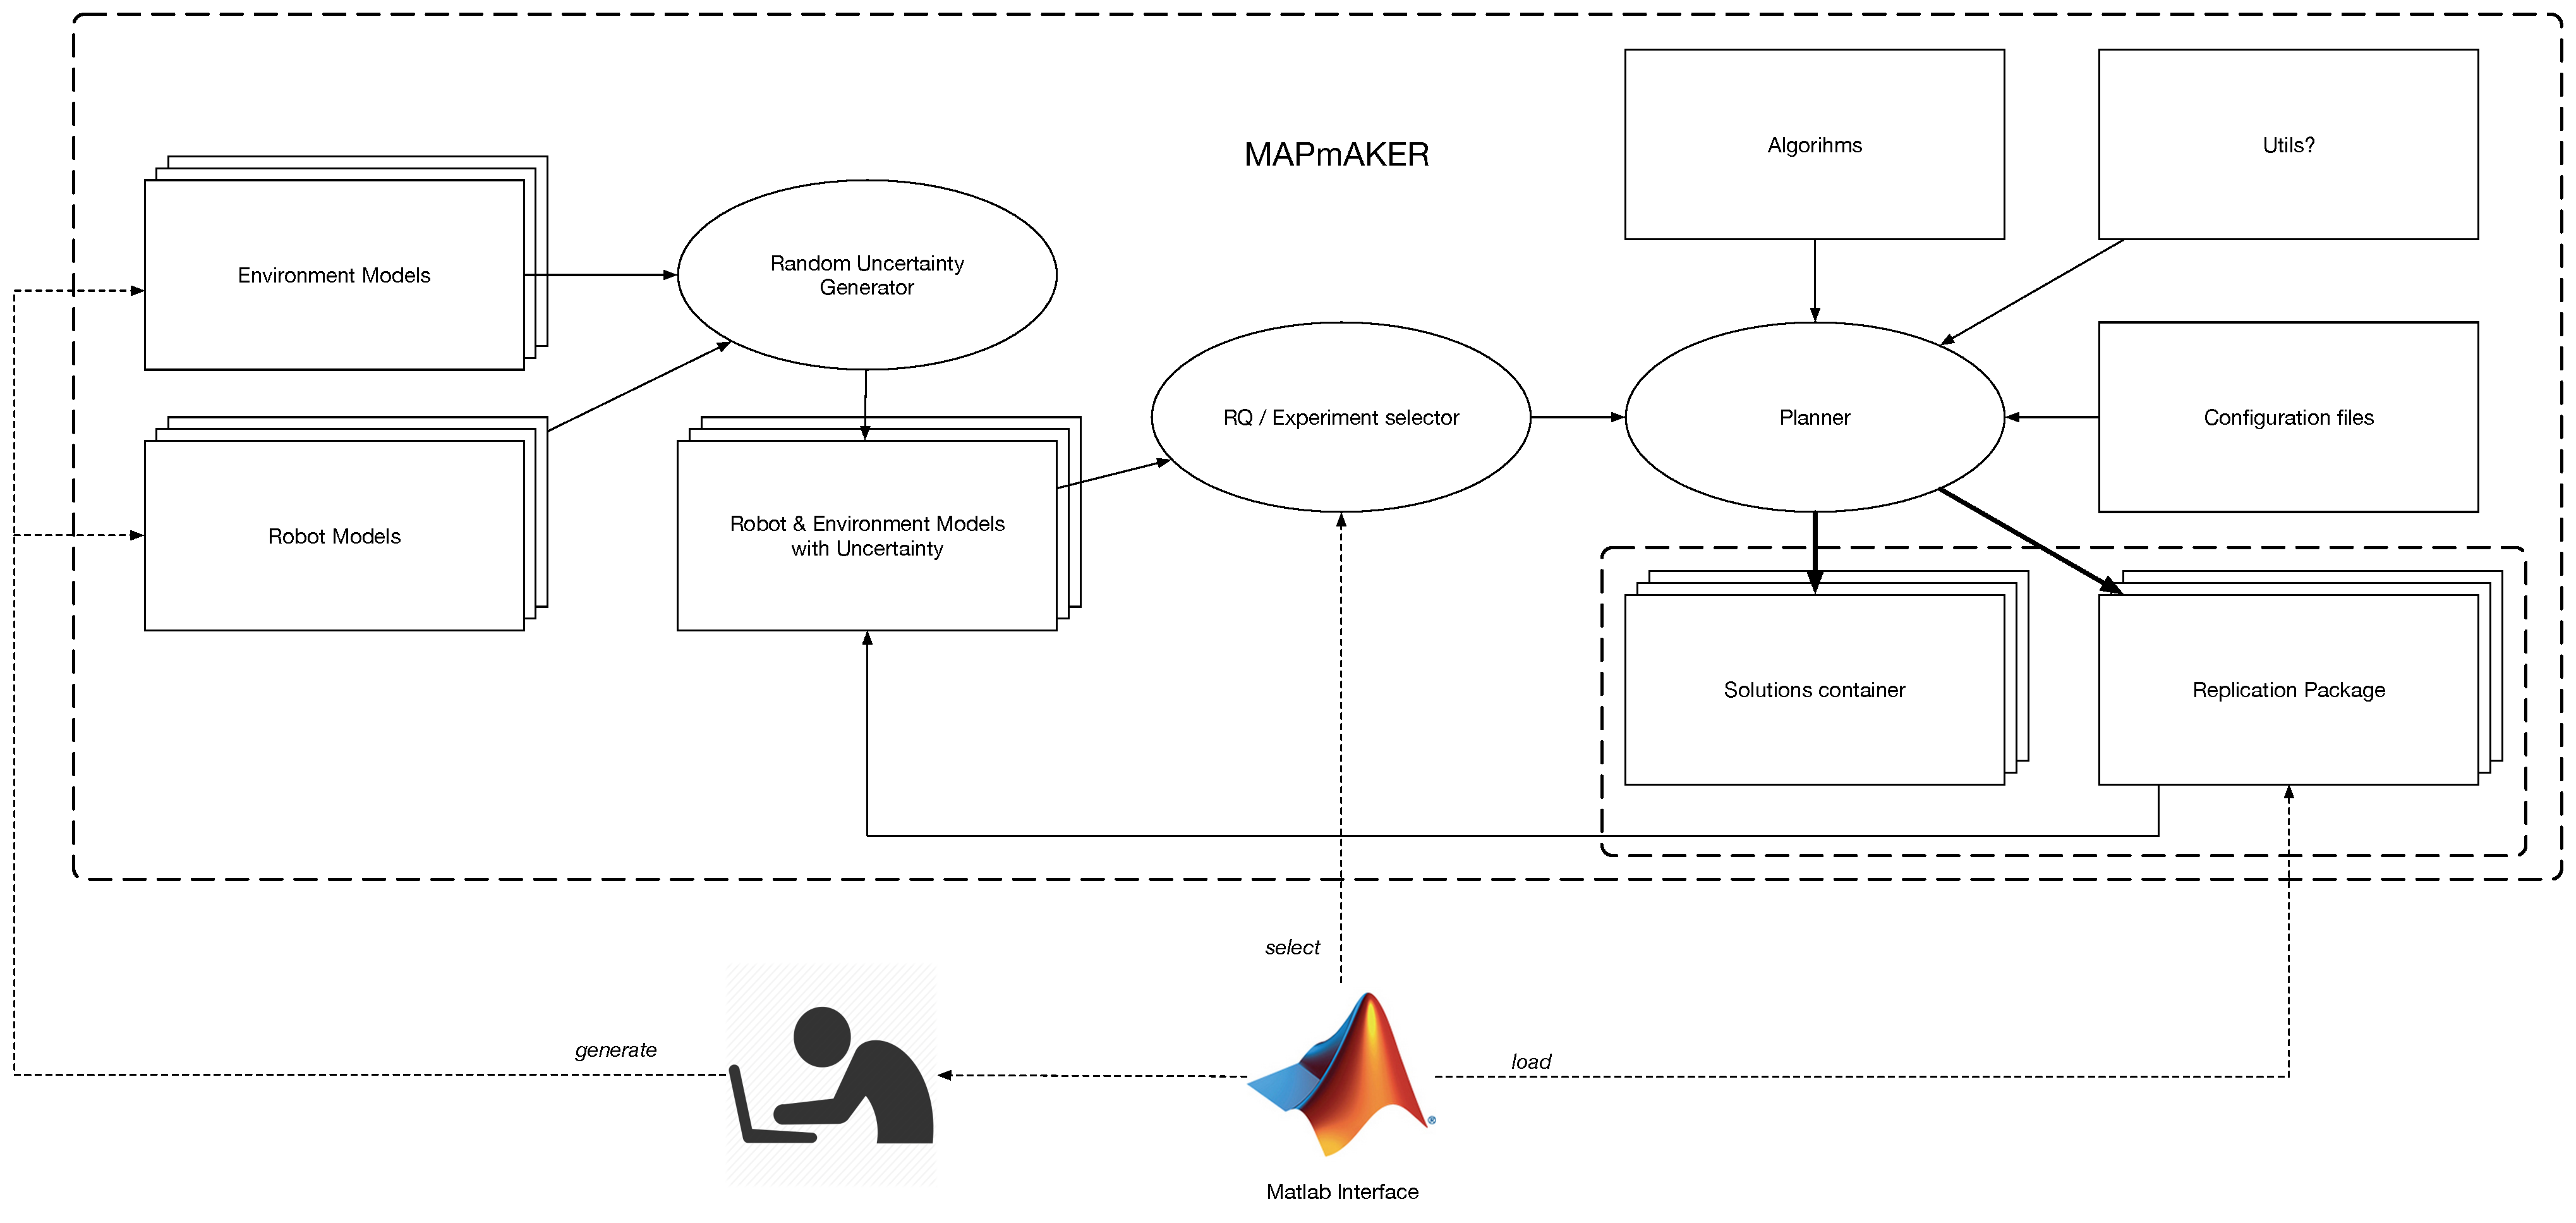
\includegraphics[width=0.9\linewidth]{Figures/MAPmAKER.pdf}
\caption{Overview of the MAPmAKER approach.}
\label{fig:overview}
\end{center}
\end{figure}





